\section{Laborfertiger Aufbau}

Der Laborfertige Aufbau wird auf Kugellagern gelagert, sowie mit einer Bremsscheibe gebremst, was ein wiederholtes Durchführen des Versuches ohne Bedenken aufgrund der entstehenden Hitze ermöglicht.

Nicht definiert sind:

\begin{itemize}
    \item Montage der Bremsbacken
    \item Montage der Wägezelle
    \item Montage des IR-Sensors
\end{itemize}

\begin{figure}[H]
    \begin{center}
        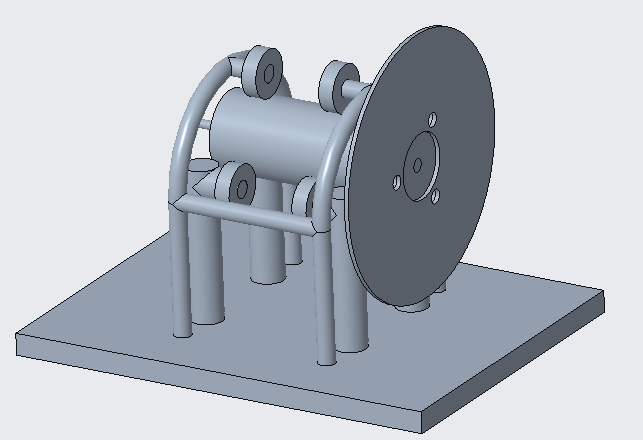
\includegraphics[width=0.3\textwidth]{versuchsaufbau2.PNG}
        \caption{3D Modell für den Laboraufbau}
    \end{center}
\end{figure}